%%%%%%%%%%%%%%%%%%%%%%%%%%%%%%%%%%%%%%%%%%%%%%%%%%%%%%%%%%%%%%%%%%%%%%%%%%%%%%%%%%
\documentclass[10pt, letterpaper]{article}
%%%%%%%%%%%%%%%%%%%%%%%%%%%%%%%%%%%%%%%%%%%%%%%%%%%%%%%%%%%%%%%%%%%%%%%%%%%%%%%%%%
\usepackage{cogsci}
\usepackage{pslatex}
\usepackage{fixltx2e}
\usepackage[natbibapa]{apacite}
\usepackage[bottom]{footmisc} %package for footnotes
\usepackage{graphics}
\usepackage{amssymb}
\usepackage{ifsym}
\usepackage{anyfontsize}
\usepackage{graphicx}
\graphicspath{
{figures/}
{../../figures/diagrams/}
{../../figures/plots/}
{../../figures/stimuli/experiment2/initial/}
{../../figures/stimuli/experiment4/selection/}
{../../figures/stimuli/experiment5/initial_marked_cropped_labeled/}
{../../figures/stimuli/experiment3/initial_marked_cropped/}
{../../figures/stimuli/experiment3/initial_selection/}
}
\usepackage[font=small]{caption}  
\usepackage[justification=centering,font=scriptsize]{subfig} %for creating panels
\usepackage[countmax]{subfloat} %for creating panels
\usepackage[USenglish]{babel}
\usepackage{gensymb}
\usepackage{booktabs} %to make nice tables
\usepackage{multirow}
\usepackage{morefloats}
\usepackage{url}
\usepackage{float}  %for floating figures
% \usepackage{fixltx2e} %fixes subscript problem
\usepackage{amsmath}
\usepackage[compact]{titlesec} %space around section headings
\usepackage{lipsum}
 \usepackage{hyperref} %remove draft option later 
\usepackage[prependcaption]{todonotes}

%nice to do notes
\newcommand{\sttodo}[2][]
{\todo[caption={\textbf{TG}}, size=\footnotesize, color = orange, #1]{#2}~}

\newcommand{\ttodo}[2][]
{\vspace{0.1cm} \hfil \todo[caption={\textbf{TG}}, size=\small, color = orange, inline, #1]{#2}}

\newcommand{\sltodo}[2][]
{\todo[caption={\textbf{LZ}}, size=\footnotesize, color = green, #1]{#2}~}

\newcommand{\ltodo}[2][]
{\vspace{0.1cm} \hfil \todo[caption={\textbf{LZ}}, size=\small, color = green, inline, #1]{#2}}

\setlength{\marginparwidth}{1.5cm}
% \usepackage{hyperref} %remove draft option later   
\hypersetup{
		colorlinks,%
		citecolor=black,%
		filecolor=black,%
		linkcolor=black,%
		urlcolor=black
}
\usepackage{multicol}%to define multiple columns

\linespread{1}

%to allow for more float figure space per page
\renewcommand\floatpagefraction{.95}
\renewcommand\topfraction{.95}
\renewcommand\bottomfraction{.95}
\renewcommand\textfraction{.05}   
\setcounter{totalnumber}{50}
\setcounter{topnumber}{50}
\setcounter{bottomnumber}{50}

% \renewcommand{\bottomtitlespace}{0pt}

%\setlength{\columnsep}{0.5cm} %column separation

%title spacing 
\titlespacing{\section}{0pt}{*0.5}{*0.5}
\titlespacing{\subsection}{0pt}{*0.5}{*0.5}
\titlespacing{\subsubsection}{0pt}{*0.1}{*1}

%for possessive citing
\def\citepos#1{\citeauthor{#1}'s (\citeyear{#1})}

%for tick marks
\usepackage{pifont}% http://ctan.org/pkg/pifont
\newcommand{\cmark}{\ding{51}}%
\newcommand{\xmark}{\ding{55}}%

%penalty for splitting footnotes
\interfootnotelinepenalty=10000

%space between footnote and text
\setlength{\skip\footins}{0.2cm}

\begin{document}

\title{Faulty Towers: A counterfactual simulation model of physical support}

\author{
\large \bf Tobias Gerstenberg, Liang Zhou, Kevin A. Smith \& Joshua B. Tenenbaum \\
\{tger, zhoul, k2smith, jbt\}@mit.edu \\
Brain and Cognitive Sciences, Massachusetts Institute of Technology
}
\maketitle
\begin{abstract}
an abstract ... 
\textbf{Keywords:} 
\end{abstract}

%%%%%%%%%%%%%%%%
% MAIN TEXT BEGINS HERE 
%%%%%%%%%%%%%%%%

\section{Introduction}

When we look at a physical scene, such as the towers shown in Figure~\ref{fig:exp1_stimuli}, we don't just see a pile of bricks. 
% We go beyond the perceptual representation of the scene in a multitude of ways. 
% We go beyond what we see in in a multiplicity of ways. 
We also have a sense for how stable the towers are, what would happen if the table got bumped in one direction or another, and what the relative masses of different bricks must be given that the tower is stable \citep{hamrick2016inferring,battaglia2013simulation}. In this paper, we show that people can not only gage the stability of the tower overall, but also judge the extent to which different bricks individually contribute to the tower's stability. We develop a \emph{counterfactual simulation model} (CSM) of physical support which determines a brick's causal responsibility for the tower's stability by simulating what would happen if the brick was removed. \sttodo{maybe talk about recent successes in deep learning with these tasks?; peter's new paper?!}

% When we see a poster depicting Michael Jordan on his way to a slam dunk (tongue sticking out of course), we represent the scene not only at this particular instance in time, but also represent what will happen next, and what happened before. That is, we represent the scene \emph{dynamically}. But how do we know what will happen next and what happened before? 

% \begin{itemize}
% 	\item handwritten characters \citep{freyd1987dynamic,lake2015human-le}
% 	\item \cite{freyd1987dynamic}: perceiving dynamic information during recognition of static handwritten forms 
% 	\item \cite{lake2015human-le}: generative model of written characters, hierarchical model with a grammar that contains of strokes and substrokes put together in a way so as to generate the intended character 
% \end{itemize}

% \begin{itemize}
% 	\item then move on to physics example 
% 	\item sometimes people have difficulty reasoning based on static stimuli \citep{mccloskey1983naive}
% 	\item sometimes it works out \citep{battaglia2013simulation}
% \end{itemize}


% \begin{itemize}
% 	\item \cite{gerstenberg2016theories,goodman2015concepts,lake2016building}
% \end{itemize}

% \subsection{Mental models and dynamic representations}
% \label{sub:mental_models_and_dynamic_representations}

% \begin{itemize}
% 	\item psychology work on simulation \citep{battaglia2013simulation,smith2013sources,hegarty2004mechanical}
% 	\item representational momentum stuff \cite{freyd1987dynamic,freyd1984representational}
% 	\item work on the perception of events: Jeffrey Zacks' work 
% \end{itemize}

% \subsection{Causal interactions and physical support}
% \label{sub:causal_interactions_and_causal_support}

% \begin{itemize}
% 	\item psychology work on physical support \citep{holmes2013spatial,freyd1988represen}
% \end{itemize}

In previous work, we showed how the counterfactual simulation model explains people's causal judgments about dynamic collision events \citep{gerstenberg2012noisy,gerstenberg2014simulation,gerstenberg2015how,gerstenberg2016almost}. In these experiments, participants saw collisions between billiard balls and they were asked to evaluate to what extent one ball had caused another ball to go through a gate in a wall (or prevented the ball from going through). The CSM assumes that people reach this judgment by comparing what actually happened with what would have happened in a counterfactual situation in which the candidate cause had been removed from the scene (or perturbed). In line with the CSM, the results of the experiments showed that there was a very close correspondence between the counterfactual judgments of one group of participants, and the causal judgments of another group. As predicted by the model, participants' cause and prevention judgments increased the more certain they were that the outcome would have been different if the candidate cause had been removed from the scene. The CSM not only predicts participants' causal judgments to a high degree of quantitative accuracy, it also captures the cognitive processes by which participants reach their judgments. Participants' eye-movements reveal how they spontaneously anticipate what would have happened in the relevant counterfactual situation \citep{gerstenberg2016tracking}. The CSM makes the strong prediction that counterfactual simulation forms a necessary part of how people make causal judgments, and that no adequate account of people's causal judgments about particular events can be developed that does not rely on counterfactuals \citep[cf.][]{wolff2007representing}. Thus far, however, the CSM has only been applied to modeling causal judgments about dynamic collision events. Here, we demonstrate the generality of the account by showing how the model naturally handles judgments about physical support. 

% The CSM predicts participants' causal judgments to a very high degree of quantitative accuracy across a wide range of situations that feature interactions with bricks and teleports \citep{gerstenberg2014simulation}, as well as multiple candidate causes \citep{gerstenberg2015how}. 
% We have also used the model to better understand when people say that A almost caused B to go through the gate \citep{gerstenberg2012noisy,gerstenberg2016almost}. 


Judging support is different from judging causation in several ways.  
% Even though the domain of interest is still people's intuitive understanding of physics, judgments about physical support differ from judgments about collisions in several respects. 
% First, while collisions events dynamically unfold over time, situations of physical support are static. That is, nothing actually happens in the scene. 
% \begin{itemize}
% 	\item notion of support is naturally expressed in terms of counterfactuals 
% 	\item part of what it means for object A to support object B, is that that object B would move (or maybe even fall) if object A weren't present 
% \end{itemize}
% The Golden Gate bridge supports the cars that drive on it. These cars would take a plunge into the sea of the bridge were to collapse. 
For example, most philosophical approaches to causation take the causal relata (i.e. the things that do the causing) to be events \citep{halpern2016causality,paul2013causation}. It is the player's kicked that caused the ball to go in the goal. 
% It is the collision event between ball A and ball B that causes ball B's going through the gate. 
However, when we consider the extent to which a particular brick is causally responsible for the tower's stability, nothing actually happens. The tower is just sitting there -- there are no events. So, rather than defining a counterfactual operation on events, CSM considers what would happen to the tower if the brick was removed. 
% simulates what would happen if the object of interest wasn't present in the scene. 
% Nevertheless, the CSM is flexible in that it can define counterfactual interventions on objects in the generative model of the scene, rather than on the events that they participated in. 
% \sttodo{maybe make the point that it's actually often more natural to define counterfactual interventions on objects}
% We can think of the causal responsibility that a brick carries for the tower's stability by considering what would happen to the tower if the brick was removed. 
The more certain we are that the tower would collapse, the more responsible the brick for its stability. 

The road map for the rest of the papers is as follows: We will first discuss the relevant background literature. Then, we present the CSM in detail. We will test the model with two experiments that ask some participants to make hypothetical judgments, and others to evaluate causal responsibility. We end by discussing limitations of the current approach, and directions for future research. 

\ttodo{signpost: what is the right counterfactual model? reference to Lewis (counterfactual most similar to the actual world); no mismatch in emphasis between introduction and rest of the paper}

% \begin{itemize}
% 	\item notion of intervention and where to apply noise
% \end{itemize}

% \begin{itemize}
% 	\item say why this is an important issue when considering counterfactuals $\rightarrow$ noise should only be applied locally (independent parts of the world should stay like they were, \citep{pearl2000causality})
% 	\item global noise applied to the scene 
% \end{itemize}

\begin{figure}[t]
\captionsetup[subfigure]{labelformat=empty}
\setlength{\fboxsep}{0pt}
\setlength{\fboxrule}{1pt}
\centering
{\hfill}
\subfloat[][]{\fbox{\includegraphics[width=0.23\columnwidth]{exp1_trial5_marked_cropped_labeled}}}
\hfill
\subfloat[][]{\fbox{\includegraphics[width=0.23\columnwidth]{exp1_trial2_marked_cropped_labeled}}}
\hfill
\subfloat[][]{\fbox{\includegraphics[width=0.23\columnwidth]{exp1_trial10_marked_cropped_labeled}}}
\hfill
\subfloat[][]{\fbox{\includegraphics[width=0.23\columnwidth]{exp1_trial14_marked_cropped_labeled}}}
{\hfill}
\vspace{-0.6cm}

{\hfill}
\subfloat[][]{\fbox{\includegraphics[width=0.23\columnwidth]{exp1_trial24_marked_cropped_labeled}}}
\hfill
\subfloat[][]{\fbox{\includegraphics[width=0.23\columnwidth]{exp1_trial28_marked_cropped_labeled}}}
\hfill
\subfloat[][]{\fbox{\includegraphics[width=0.23\columnwidth]{exp1_trial22_marked_cropped_labeled}}}
\hfill
\subfloat[][]{\fbox{\includegraphics[width=0.23\columnwidth]{exp1_trial41_marked_cropped_labeled}}}
{\hfill}
\vspace{-0.6cm}
\caption{\textbf{Experiment~1}. Example stimuli. \emph{Note}: Red bricks that would fall off the table if the black brick were removed (according to ground truth) are marked with a white dot at their center. The dots were not displayed in the actual experiment.}
\label{fig:exp1_stimuli}
\end{figure}


\subsection{A counterfactual simulation model of physical support}

%  \begin{itemize}
% 	\item talk about how the model needs to be adapted to capture judgments of physical support 
% 	\item different ways of capturing people's uncertainty\footnote{An interface to see the stimuli and play around with different noise models can be accessed here: \url{link_to_interface}} 
% \end{itemize}

% \begin{itemize}
% 	\item what's the relevant situation
% 	\item what would have happened in that situation ...
% \end{itemize}

In our experiments, we ask participants how responsible the black brick is for the red bricks staying on the table. 
To derive predictions from the CSM we need to determine (1) what counterfactual situation to consider, and (2) how to simulate what would happen in that situation. We assume that when judging responsibility, participants consider a counterfactual situation in which the black brick was removed. Participants then use their intuitive understanding of physics to mentally simulate what would happen in that situation.\footnote{We use the term \emph{counterfactual} here broadly to refer to a possible world that

simulation model to highlight similarities to the model we developed for dynamic collision events. However, when judging 

responsibility for support participants need not go back in time to think about what would have happened, but merely need to consider the \emph{hypothetical} of what would happen if the brick was removed.}
\ttodo{footnote here needs to be updated}


While some work suggests that people's understanding of the physical world is systematically biased \citep{mccloskey1983naive}, recent work has argued that some aspects of people's intuitive understanding of physics is well-described by making the assumption that people have an approximate simulation engine in their mind that is akin to a physics engine that generates physically realistic scenes \citep{battaglia2013simulation,lake2016building}. Part of what makes these simulation engines in the mind ``approximate'' is that they assume that people's representation of a physical situation is uncertain. This uncertainty can come in many forms, such as perceptual uncertainty about the exact location of objects \citep{battaglia2013simulation}, dynamic uncertainty about how exactly an object will move \citep{smith2013sources}, and uncertainty about latent physical parameters such as friction and mass \citep{sanborn2013reconciling}. For example, in \citepos{battaglia2013simulation} experiments, participants were asked to say whether a tower was stable, or in which direction a tower would fall. They modeled people's uncertainty by running many noisy simulations of the actual scene in which the position of the bricks was slightly perturbed. Participants' stability judgments were highly correlated with the average proportion of bricks that fell across these noisy simulations.  

We contrast three different implementations of the CSM which differ in terms of how they capture people's uncertainty about what would have happened if the black brick had been removed. All models apply noise in the same way: as a small impulse to the red bricks very shortly after the black brick was removed.\sttodo{say more about how this impulse is applied} However, the models differ in which bricks they apply noise to when simulating the relevant counterfactual. Figure~\ref{fig:noise_model_diagrams} illustrates how the three different models work. The \emph{global noise} model applies a small impulse to all the bricks. The \emph{local noise} model applies the impulse only to the red bricks that are directly in contact with the black brick. The \emph{above noise} model applies noise only to bricks that are above the black brick and connected with it. To determine which bricks are connected it first looks at which bricks are directly in contact with the black brick \emph{and} above it.\sttodo{enter some more explanation by what we mean by ``above''} It then recursively applies the same criterion to the identified red bricks. That is, it then looks at what other bricks are in contact with the identified red bricks, and above them. For example, brick 2 in Figure~\ref{subfig:noise_local_above} is subject to noise since brick 1 is in contact and above the black brick, and brick 2 is in contact and above brick 1. The local noise models incorporate the assumption that only some aspects of the physical scene would be directly affected by the counterfactual intervention. Those aspects of a situation that are completely disconnected from the counterfactual intervention should remain exactly as they were. We test this assumption directly in Experiment~2 which features disjoint configurations of bricks (cf. Figure~\sttodo{insert figure reference}).

\begin{figure}[t]
\centering
{\hfill}
\subfloat[][global noise]{\label{subfig:noise_global}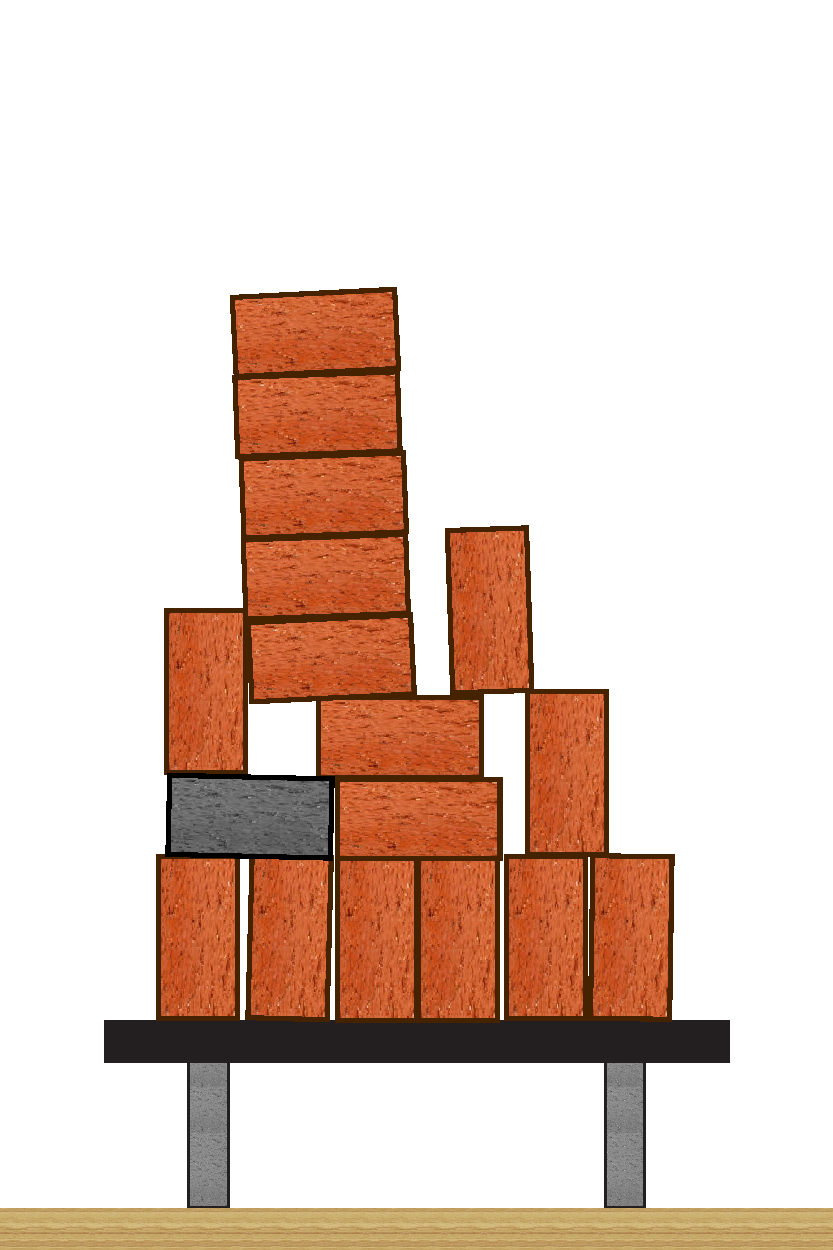
\includegraphics[width=0.3\columnwidth]{noise_global}}
\hfill
\subfloat[][local noise]{\label{subfig:noise_local}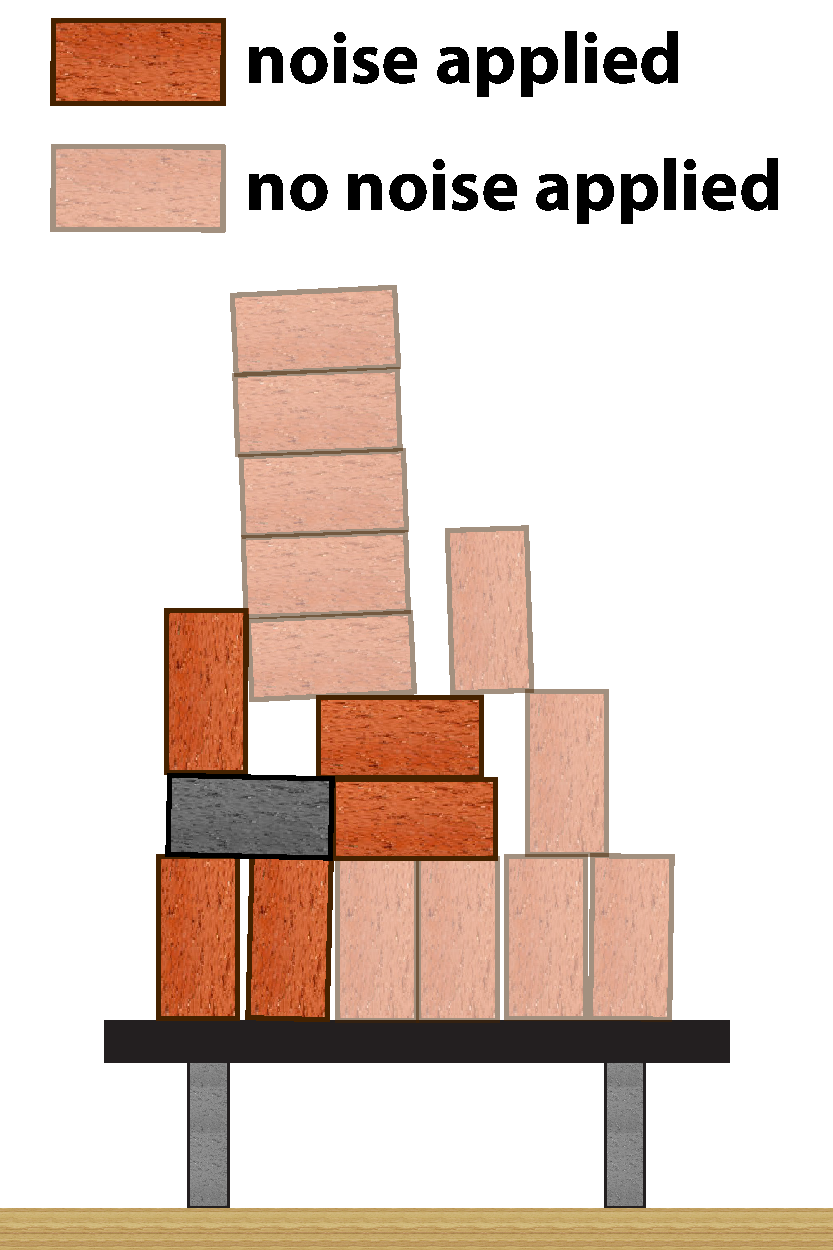
\includegraphics[width=0.3\columnwidth]{noise_local}}
\hfill
\subfloat[][above noise]{\label{subfig:noise_local_above}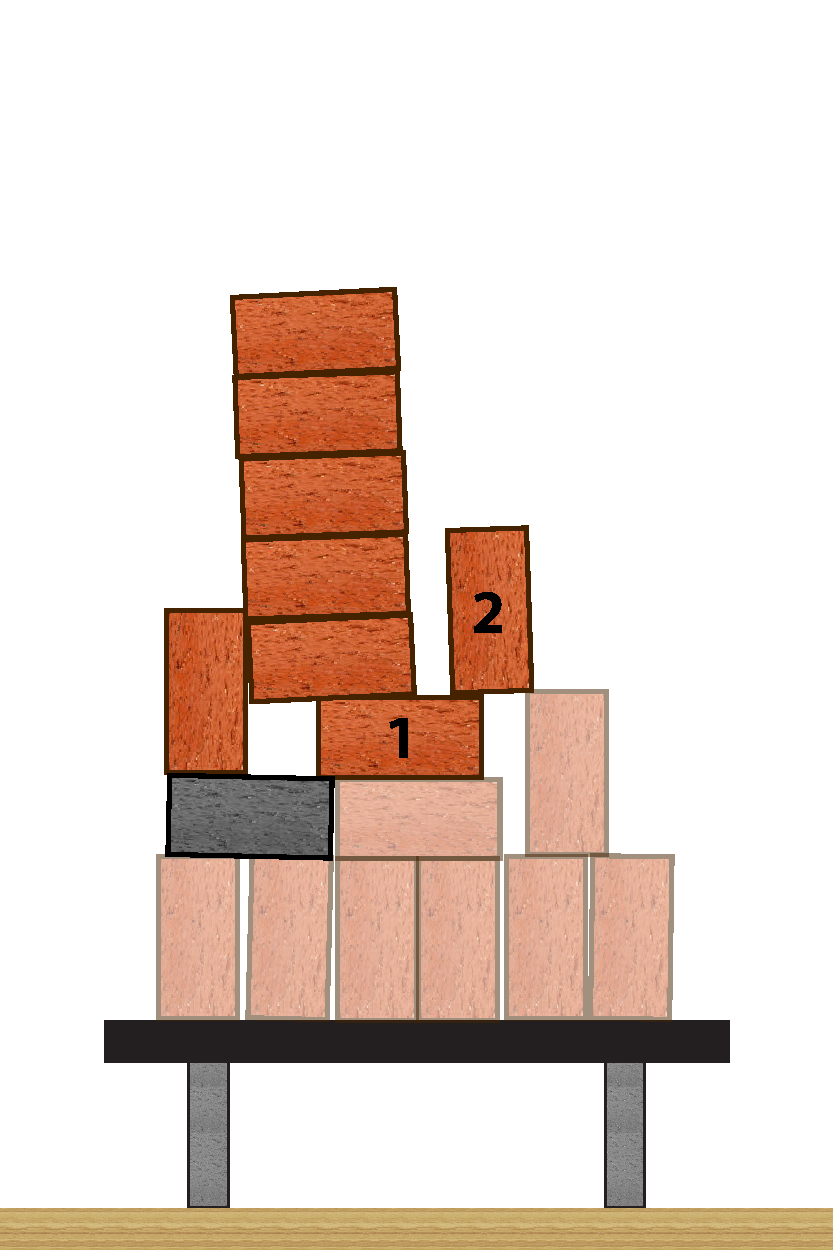
\includegraphics[width=0.3\columnwidth]{noise_local_above}}
{\hfill}
\vspace{-0.2cm}
\caption{Schematic illustration of how different versions of the counterfactual simulation model apply noise when considering what would happen if the black brick were removed. The opacity of the red bricks indicates for each version of the model which bricks were subjected to noise.}
\label{fig:noise_model_diagrams}
\ttodo{maybe add some more numbers to the loca-above model to explain why some bricks are not included}
\end{figure}

\section{Experiment 1}
\label{sec:experiment_1}

In the experiment, participants saw towers of bricks like the ones shown in Figure~\ref{fig:exp1_stimuli}. Depending on the experimental condition, participants were asked to consider what would happen if the black brick wasn't there, or evaluate the extent to which the black brick is responsible that the red bricks stay on the table. In line with the CSM, we predicted that there would be a close relationship between counterfactual and responsibility judgments. 

\subsection{Methods}
\label{sub:methods}

\subsubsection{Design \& Procedure}

The experiment had three experimental conditions that only differed in terms of the dependent measure. In the \emph{prediction condition}, participants were asked to answer the question: ``How many of the red bricks would fall off the table, if the black brick wasn't there?'' Participants provided their answer on a sliding scale ranging from 0 to the number of red bricks present in the scene in steps of 1. In the \emph{selection condition}, participants were asked to ``Please click on the red bricks that would fall off either side of the table if the black brick wasn't there.'' In the \emph{responsibility condition}, participants were asked to answer the question: ``How responsible is the black brick for the red bricks staying on the table?'' Responses were provided on a sliding scale ranging from ``not at all'' (0) to ``very much'' (100). 
%The slider only appeared once participants clicked on the sliding scale. 

The procedure for all three conditions was identical. Participants first received instructions about the task. They then saw a number of animations that showed 20 bricks being dropped on the table.\footnote{We used the same methodology to generate the stimuli for Experiment~1.} These animations were shown so as to familiarize participants with the relevant properties of the physical scene such as the bricks' mass, the friction between the bricks, as well as the table friction. Participants were allowed to proceed to the next stage once they had watched at least five animations. 

After the familiarization, participants saw 42 images of different towers of bricks in randomized order (see Figure~\ref{fig:exp1_stimuli} for examples). The stimuli varied the number of bricks on the table (range = 7 to 20, M = 13.7, SD = 3.3), as well as the number of red bricks that would fall off the table if the black brick was removed (range = 0 to 6, M = 2, SD = 1.9). Participants' task differed depending on the condition as described above. Finally, participants were asked to give open-ended feedback about the task, and provided demographic information. 

On average, the experiment took 9.86 (SD = 6.49), 15.71 (SD = 6.49), and 8.88 minutes (SD = 8.90) in the prediction, selection, and responsibility condition, respectively. \sttodo{if there is space/time, make a diagram that illustrates the three different conditions}

\subsubsection{Participants}
121 participants (M\textsubscript{age} = 34, SD\textsubscript{age} = 12, 47 female) were recruited via Amazon Mechanical Turk with $N = 42$ in the prediction condition, $N = 38$ in the selection condition, and $N = 41$ in the responsibility condition. We excluded participants from further analysis based on their responses to the catch trial shown in Figure~\ref{fig:exp1_stimuli}a. 11 participants in the prediction condition were excluded because they predicted that at least one red brick would fall. 6 participants in the responsibility condition were excluded because they gave a responsibility rating greater than 15 (on a scale from 0 to 100). No participants were excluded from the selection condition because no participant selected any of the bricks on the catch trial.\sttodo{rating greater than 15 sounds a little arbitrary...} 

\subsection{Results}
\label{sub:results}

We will discuss the results from the \emph{selection}, \emph{prediction}, and \emph{responsibility} conditions in turn. 

\subsubsection{Selection condition}
\label{ssub:selection_condition}

\begin{figure}[H]
\captionsetup[subfigure]{labelformat=empty}
\centering
{\hfill}
\subfloat[][]{\label{subfig:exp1_selection_ground truth_scatter}\includegraphics[width=0.48\columnwidth]{{{exp1_selection_ground_truth_scatter}}}}
\hfill
\subfloat[][]{\label{subfig:exp1_selection_impulse-global_6.9_0.5_scatter}\includegraphics[width=0.48\columnwidth]{{{exp1_selection_impulse-global_6.9_0.5_scatter}}}}
{\hfill}

\vspace{-0.5cm}

{\hfill}
\subfloat[][]{\label{subfig:exp1_selection_impulse-local_11.2_0.5_scatter}\includegraphics[width=0.48\columnwidth]{{{exp1_selection_impulse-local_11.2_0.5_scatter}}}}
\hfill
\subfloat[][]{\label{subfig:exp1_selection_impulse-local-above-extended_14.3_0.5_scatter}\includegraphics[width=0.48\columnwidth]{{{exp1_selection_impulse-local-above-extended_14.3_0.5_scatter}}}}
{\hfill}
\vspace{-0.5cm}
\caption{\textbf{Experiment 1}. Scatter plots showing the relationship between the empirical probability with which each brick was selected and the (a) ground truth as well as the predictions of the best-fitting (b) global noise model, (c) local noise model, and (d) above noise model.}
\label{fig:exp1_selection_models}
\end{figure}

\ttodo{also test a regression model with features ... }

We tested how well the three noise models described above captured participants' selections of which bricks would fall off the table if the black brick wasn't there (see Figure~\ref{fig:noise_model_diagrams}). 
% For each model, we generated searched over a range of the noise parameter that determines the strength of the impulse applied to the different bricks. 
For each model, we used maximum likelihood fitting to find the the noise parameter which predicts participants' selections best. For each setting of the noise parameter, we ran 100 simulations per stimulus and used the proportion of samples that each brick fell off the table in the noisy simulations to predict the probability that a given brick will be selected to fall by participants.\footnote{Figure~\ref{fig:exp2_model_comparison} gives an example for what these predictions look like for stimuli used in Experiment~2.}

Figure~\ref{fig:exp2_model_comparison} shows how well the different noise models account for participants' selections. Overall, the \emph{above noise} model accounts best for the data (cf. Table~\ref{tab:model_results}). 

\begin{table}[b]
\caption{Summary of model results for Experiments 1 and 2 as applied to the data in the \emph{selection condition}.}
\label{tab:model_results}
\vspace{-0.2cm}
\centering
% \setlength\tabcolsep{0.1cm}
% {\fontsize{8}{10}\selectfont
\resizebox{\columnwidth}{!}{\begin{tabular}{r|cccc|cccc}
  \toprule
  & \multicolumn{4}{c}{\textbf{Experiment 1}} & \multicolumn{4}{c}{\textbf{Experiment 2}} \\
model & r & RMSE & L & $\sigma$ & r & RMSE & L & $\sigma$\\ 
  \midrule
truth & 0.55 & 34.74 & -21374 & 0 & 0.64 & 31.65 & -22279 & 0 \\ 
    global & 0.75 & 20.92 & -9274 & 6.9 & 0.61 & 29.03 & -14034 & 2.5 \\ 
    local & 0.70 & 22.26 & -9727 & 11.2 & 0.66 & 25.35 & -12617 & 7.2 \\ 
    above & 0.87 & 15.34 & -8435 & 14.3& 0.73 & 22.08 & -11824 & 12.5 \\ 
   \bottomrule
\end{tabular}
}
{\fontsize{8}{9}\selectfont 
\begin{flushleft}
\emph{Note:}  r = Pearson correlation, RMSE = root mean squared error, L = log-likelihood of the data, $\sigma$ = SD of the Gaussian from which the noise impulse is drawn.
\end{flushleft}
}
\end{table}

\subsubsection{Prediction condition}
\label{ssub:prediction_condition}

\begin{figure}[H]
%\captionsetup[subfigure]{labelformat=empty}
\centering
{\hfill}
\subfloat[][\textbf{Experiment 1}]{\label{subfig:exp1_prediction_selection_scatter}\includegraphics[width=0.48\columnwidth]{exp1_prediction_selection_scatter}}
\hfill
\subfloat[][\textbf{Experiment 2}]{\label{subfig:exp2_prediction_selection_scatter}\includegraphics[width=0.48\columnwidth]{exp2_prediction_selection_scatter}}
{\hfill}
\vspace{-0.2cm}
\caption{Relationship between the predicted number of red bricks that would fall if the black brick wasn't there (prediction condition) and number of selected bricks that would fall (selection condition). \emph{Note}: The letters refer to the examples shown in Figure~\ref{fig:exp1_stimuli} for Experiment~1, and Figure~\ref{fig:exp2_stimuli} for Experiment~2. Error bars denote bootstrapped 95\% confidence intervals.}
\label{fig:prediction_selection_scatter}
\end{figure}

Figure~\ref{fig:prediction_selection_scatter} shows the relationship between the number of bricks predicted to fall, and the average number of bricks that participants selected in the selection condition. Overall, the two ways of probing participants' counterfactual simulations lead to very similar results. However, participants in the prediction condition predicted that more bricks would fall than participants in the selection condition selected (most of the data points are below the diagonal). 

The noise model which best accounted for participants' selections, also accurately predicts participants' average judgments about how many bricks would fall with $r = , \text{RMSE} = $.\sttodo{needs to be updated once final simulations have been run} 

\subsubsection{Responsibility condition}
\label{ssub:responsibility_condition}

\begin{figure}[H]
\centering
{\hfill}
\subfloat[][\textbf{Experiment 1}]{\label{subfig:exp1_prediction_responsibility_scatter}\includegraphics[width=0.48\columnwidth]{exp1_prediction_responsibility_scatter}}
\hfill
\subfloat[][\textbf{Experiment 2}]{\label{subfig:exp2_prediction_responsibility_scatter}\includegraphics[width=0.48\columnwidth]{exp2_prediction_responsibility_scatter}}
{\hfill}
\vspace{-0.2cm}
\caption{Relationship between the predicted proportion of bricks that would fall if the black brick wasn't there and responsibility judgments. \emph{Note}: The letters refer to the examples shown in Figure~\ref{fig:exp1_stimuli} for Experiment~1, and Figure~\ref{fig:exp2_stimuli} for Experiment~2. Error bars denote bootstrapped 95\% confidence intervals.}
\label{fig:prediction_responsibility_scatter}
\ttodo{maybe have the same axis ranges?}
\end{figure}

Figure~\ref{subfig:exp1_prediction_responsibility_scatter} shows the relationship between the proportion of bricks that participants in the \emph{prediction condition} believed would fall off the table if the black brick wasn't present in the scene, and participants' responsibility judgments. As predicted by the CSM, there was a very high quantitative relationship between counterfactual and responsibility judgments. This strongly suggests that participants evaluated a brick's responsibility by considering what proportion of bricks would have fallen off the table if the brick hadn't been there. When we use the proportion of bricks selected in the \emph{selection condition}  to predict participants responsibility judgments, we get a similarly good fit with $r = .78$, $\text{RMSE} = 7.65$. Finally, we can also use the best-fitting noise model to account for participants' responsibility judgments with $r = .78$, $\text{RMSE} = 7.65$. We will discuss the fact that responsibility judgments are more closely related to the prediction judgments compared to the selections in the General Discussion.

\subsection{Discussion}
\label{sub:discussion}

The results of Experiment~1 support the predictions of the CSM. Most importantly, there was a very close relationship between the responsibility judgments of one group of participants, and the number of bricks that another group of participants predicted would fall if the black brick wasn't there. We contrasted three instantiations of the CSM the differ in the way in which they capture people's uncertainty about what would happen if the brick was removed. The results show that the \emph{above model} explains participants' selections best. 


% \begin{itemize}
% 	\item models were overall relatively highly correlated 
% 	\item since all the stimuli were different, it is in principle possible that participants could have answered the question by focusing on a number of features 
% 	\item Experiment~2 provides a more controlled setup that also helps to better distinguish between local and global noise models 
% \end{itemize}

\sttodo{maybe Liang can have another look through the participants' comments and mark interesting ones}

\section{Experiment 2}
\label{sec:experiment_2}

One limitation of Experiment~1 is that the predictions of the different noise models are highly correlated with each other. For example, the correlation between the \emph{above} and \emph{global} model is $r = $.\sttodo{enter correlation here} Experiment~1 elicited participants' judgments for a wide array of different situations. In Experiment~2, we generated a smaller subset of situations that were more tightly controlled. 

\begin{itemize}
	\item experiment that distinguishes between the different models 
	\item illustrate the locality point by talking through 3 concrete examples 
\end{itemize}

\subsection{Methods}
\label{sub:methods}

\subsubsection{Design \& Procedure}
\label{ssub:design_&_procedure}

\begin{figure}[H]
\captionsetup[subfigure]{labelformat=empty}
\setlength{\fboxsep}{0pt}
\setlength{\fboxrule}{1pt}
\centering
{\hfill}
\subfloat[][]{\fbox{\includegraphics[width=0.23\columnwidth]{trial8_marked_cropped}}}
\hfill
\subfloat[][]{\fbox{\includegraphics[width=0.23\columnwidth]{trial2_marked_cropped}}}
\hfill
\subfloat[][]{\fbox{\includegraphics[width=0.23\columnwidth]{trial17_marked_cropped}}}
\hfill
\subfloat[][]{\fbox{\includegraphics[width=0.23\columnwidth]{trial18_marked_cropped}}}
{\hfill}
\vspace{-0.6cm}

{\hfill}
\subfloat[][]{\fbox{\includegraphics[width=0.23\columnwidth]{trial26_marked_cropped}}}
\hfill
\subfloat[][]{\fbox{\includegraphics[width=0.23\columnwidth]{trial33_marked_cropped}}}
\hfill
\subfloat[][]{\fbox{\includegraphics[width=0.23\columnwidth]{trial42_marked_cropped}}}
\hfill
\subfloat[][]{\fbox{\includegraphics[width=0.23\columnwidth]{trial21_marked_cropped}}}
{\hfill}
\vspace{-0.6cm}
\caption{\textbf{Experiment~2}. Example stimuli. \emph{Note}: The white dots indicate which bricks would fall if the black brick wasn't there. There were 6 different configurations of towers, and 7 different positions for the black brick in each tower, see c), d), and h).}
\ttodo{can remove the subtitles by adding text to the figures directly}
\label{fig:exp2_stimuli}
\end{figure}

Figure~\ref{fig:exp2_stimuli} shows a selection of the stimuli. We generated six different tower configurations. For each tower, we chose seven different positions for the black brick. Figure~\ref{fig:exp2_stimuli}c, d, and g show three examples for the position of the black brick for this configuration. The towers and brick positions were chosen such that removing the black brick would lead to 0--6 bricks falling off the table for the seven different instances of each tower configuration. Furthermore, as mentioned above, we included configurations which featured disjointed sets of bricks, such as Tower III and Tower IV. 

The procedure was identical to that of Experiment~1. On average, the experiment took 11.57 (SD = 5.24), 13.04 (SD = 6.87), and 7.86 minutes (SD = 3.48) in the prediction, selection, and responsibility condition, respectively. 

\ttodo{maybe make the point that participants in the responsibility condition were pretty fast, so it's likely that they didn't think through each individual brick}

\subsubsection{Participants}
\label{ssub:participants}
129 participants (M\textsubscript{age} = 36, SD\textsubscript{age} = 11.3, 59 female) were recruited via Amazon Mechanical Turk with $N = 42$ in the prediction condition, $N = 44$ in the selection condition, and $N = 43$ in the responsibility condition. Using the same stimulus and exclusion criteria as in Experiment~1, 3 participants were removed in the prediction condition, 1 in the selection condition, and 3 in the responsibility condition. 

\subsection{Results}
\label{sub:results}

Again, we will discuss the results in the \emph{selection}, \emph{prediction}, and \emph{responsibility} condition in turn. 

\subsubsection{Selection condition}
\label{ssub:selection_condition}

\begin{figure}[H]
\captionsetup[subfigure]{labelformat=empty}
\centering
{\hfill}
\subfloat[][]{\label{subfig:exp2_selection_ground truth_scatter}\includegraphics[width=0.48\columnwidth]{{{exp2_selection_ground_truth_scatter}}}}
\hfill
\subfloat[][]{\label{subfig:exp2_selection_impulse-local_7.2_0.5_scatter}\includegraphics[width=0.48\columnwidth]{{{exp2_selection_impulse-local_7.2_0.5_scatter}}}}
{\hfill}

\vspace{-0.5cm}

{\hfill}
\subfloat[][]{\label{subfig:exp2_selection_impulse-global_2.5_0.5_scatter}\includegraphics[width=0.48\columnwidth]{{{exp2_selection_impulse-global_2.5_0.5_scatter}}}}
\hfill
\subfloat[][]{\label{subfig:exp2_selection_impulse-local-above-extended_12.5_0.5_scatter}\includegraphics[width=0.48\columnwidth]{{{exp2_selection_impulse-local-above-extended_12.5_0.5_scatter}}}}
{\hfill}
\vspace{-0.5cm}
\caption{\textbf{Experiment~2}: Scatter plots showing the relationship between the empirical probability with which each brick was selected and the (a) ground truth as well as the predictions of the best-fitting (b) global noise model, (c) local noise model, and (d) above noise model.}
\label{fig:exp2_selection_models}
\end{figure}

Figure~\ref{fig:exp2_selection_models} shows the correspondence between participants' brick selections and the predictions according to the ground truth as well as our three noise models as illustrated in Figure~\ref{fig:noise_model_diagrams}. Across all the stimuli, there were 564 bricks in total. Overall, the \emph{above noise} model accounts for participants' selections best. Table~\ref{tab:model_results}.


\begin{figure}[H]
\setlength{\fboxsep}{0pt}
\setlength{\fboxrule}{1pt}
\centering
{\hfill}
\subfloat[][selection]{\fbox{\includegraphics[width=0.23\columnwidth]{{{exp5_freq_trial_17_cropped}}}}}
\hfill
\subfloat[][global noise]{\fbox{\includegraphics[width=0.23\columnwidth]{{{exp5_impulse-global_2.5_0.5_trial_17_cropped}}}}}
\hfill
\subfloat[][local noise]{\fbox{\includegraphics[width=0.23\columnwidth]{{{exp5_impulse-local_7.2_0.5_trial_17_cropped}}}}}
\hfill
\subfloat[][above noise]{\fbox{\includegraphics[width=0.23\columnwidth]{{{exp5_impulse-local-above-extended_12.5_0.5_trial_17_cropped}}}}}
{\hfill}
\vspace{-0.2cm}

{\hfill}
\subfloat[][selection]{\fbox{\includegraphics[width=0.23\columnwidth]{{{exp5_freq_trial_42_cropped}}}}}
\hfill
\subfloat[][global noise]{\fbox{\includegraphics[width=0.23\columnwidth]{{{exp5_impulse-global_2.5_0.5_trial_42_cropped}}}}}
\hfill
\subfloat[][local noise]{\fbox{\includegraphics[width=0.23\columnwidth]{{{exp5_impulse-local_7.2_0.5_trial_42_cropped}}}}}
\hfill
\subfloat[][above noise]{\fbox{\includegraphics[width=0.23\columnwidth]{{{exp5_impulse-local-above-extended_12.5_0.5_trial_42_cropped}}}}}
{\hfill}
\vspace{-0.2cm}
\caption{Empirical selection percentages for two different stimuli together with the predicted selection probabilities according to the different noise models.}
\label{fig:exp2_model_comparison}
\end{figure}

Let us discuss the two situations shown in Figure~\ref{fig:exp2_model_comparison} in some more detail. For the example shown in the top row, participants are confident that only the two bricks above the black one would fall (only very few participants selected any of the other bricks). As Figure~\ref{fig:exp2_stimuli}c shows, participants' selections correspond closely to the ground truth in this case. Since the \emph{global noise} model applies an impulse to all the bricks, it incorrectly predicts that bricks on the right would fall. In contrast, the \emph{local noise} model correctly predicts that none of the bricks on the right will fall. However, since the model applies an impulse to all the bricks that are in contact with the black brick, it overpredicts that the bricks underneath the black brick would fall. The \emph{above noise}  model predicts participants' selection best in this case. It only assigns a small probability that any of the bricks on the right would fall (because sometimes the bricks on top of the black brick will fall towards the right), and a small probability that any of the bricks underneath the black brick would fall. 

The example in the bottom row shows a situation where participants' selections didn't correspond to the ground truth. Here, the majority of participants believed that none of the bricks would fall if the black brick wasn't there. However, as Figure~\ref{fig:exp2_stimuli}g shows, there are in fact six bricks that would fall according to the ground truth. When the black brick is removed, the two bricks directly underneath it fall to the left and right, and the one falling to the right pushes the stack of bricks on the right off the table. None of our noise models is able to capture participants' selections in this case. The \emph{above noise} model does a particularly poor job for the simple reason that it doesn't apply any noise in this case. Since the black brick is on top, its predictions correspond to the ground truth. What this clearly shows is that our noise models don't yet completely capture participants' counterfactual simulations. We will discuss some ideas about how the improve the models in the General Discussion below. 


\subsubsection{Prediction condition}
\label{ssub:prediction_condition}


\subsubsection{Responsibility condition}
\label{ssub:responsibility_condition}

\subsection{Discussion}
\label{sub:discussion}

\begin{itemize}
	\item maybe show some examples for where the different noise models still get things wrong (and show images that display the percentage with which each brick was selected and predicted)
\end{itemize}

\section{General Discussion}

Most importantly, the results of both experiments showed that there was very close relationship between the counterfactual judgments of one group of participants, and the responsibility judgments of another group of participants. 

\begin{itemize}
	\item maybe combine small local noise with above noise ... 
	\item make the point here that the model is ``counterfactual'' only in the lose sense; it doesn't require going back in time (so it's rather a ``hypothetical'' simulation model)
	\item maybe include a participant's comment here
	\begin{itemize}
	 	\item ``Playing angry birds helps on this, I can kind of visualize the falling bricks.''
	 	\item ``How many bricks were on top of the black brick and what would happen if it were removed. If most of the bricks would fall off the table I figured it was more important. Also if the black brick was at the top I figured it was less important and had less impact.''
	 \end{itemize} 
\end{itemize}

\fontsize{9}{11}\selectfont{
\noindent \textbf{Acknowledgments} This work was supported by the Center for Brains, Minds \& Machines (CBMM), funded by NSF STC award CCF-1231216 and by an ONR grant N00014-13-1-0333.
}

\bibliographystyle{apacite}
\def\thebibliography#1{\section*{References}
\fontsize{7}{8}\selectfont
 \list
 {[\arabic{enumi}]}{\leftmargin \parindent
	 \itemindent -\parindent
	 \itemsep 0ex plus 1pt
	 \parsep 0.2ex plus 1pt minus 1pt
	 \usecounter{enumi}}
	 \def\newbrick{\hskip .11em plus .33em minus .07em}
	 \sloppy\clubpenalty4000\widowpenalty4000
	 \sfcode`\.=1000\relax}

% \bibliography{references}
\bibliography{/Users/tobi/Documents/work/latex/TobisPapers}

\clearpage 

\section{To do list}
\label{sec:to_do_list}

\begin{itemize}
	\item ``were removed'' or ``was removed''?
	\item run regression models with features
	\item look for best-fitting models for Experiment~2
	\item test a model that combines local with local-above noise 
\end{itemize}

\section{Literature review}
\label{sec:literature_review}

\subsection{\cite{freyd1987dynamic}}

\begin{itemize}
	\item sensitive to implicit dynamic information even when they are not able to observe real-time change 
	\item perception requires information about \emph{transitions} 
	\item \emph{dynamic} mental representations: temporal dimension is necessary part of it 
	\item representational momentum 
	\item dynamic information about possible past and future $\rightarrow$ no explicit mention of counterfactuals 
\end{itemize}


\end{document}